\documentclass{article}
\usepackage[utf8]{inputenc}
\usepackage{geometry}
\geometry{margin=1in}
%\usepackage{appendix}
\usepackage{amsmath}
\usepackage{amssymb}
\usepackage[ruled,vlined, linesnumbered]{algorithm2e}
\usepackage[english]{babel}
\usepackage[nottoc]{tocbibind}
\usepackage{xcolor}
\usepackage{natbib}
\usepackage{graphicx}
\usepackage{float}
\usepackage{booktabs}
\usepackage{epstopdf}% To incorporate .eps illustrations using PDFLaTeX, etc.
\usepackage{hyperref}
\hypersetup{colorlinks=true, citecolor=black, linkcolor=., urlcolor=cyan}
\newtheorem{theorem}{Theorem}[section]
\bibliographystyle{ims}
\graphicspath{{plots/}}

% Custom commands / shortcuts
\providecommand{\sign}{\textrm{sign}}
\providecommand{\pb}[1]{\textcolor{red}{#1}}
\providecommand{\lam}{\lambda}
\newcommand{\quotes}[1]{``#1''}


\title{Adaptive Hybrid Screening for Efficient Lasso Optimization}
\author{Chuyi Wang\\Department of Statistics and Actuarial Sciences\\University of Iowa
  \and
  Patrick Breheny\\Department of Biostatistics\\University of Iowa}
\date{}

\begin{document}

\maketitle

\begin{abstract}
Lasso type models are a popular approach for analyzing high-dimensional data. The size of modern data sets can be quite large, so developing efficient algorithms is important. Feature screening techniques have proven to be effective at increasing efficiency, as they allow for considerable dimension reduction during the optimization process. In this paper, we develop an adaptive hybrid screening framework where screening is carried out adaptively along the path of tuning parameter values, reusing previous solutions to reduce heavy screening computations if they fail to significantly reduce dimensionality. We focus on the standard lasso model and sparse logistic model, but the proposed framework is flexible and can be easily extended to different types of lasso models. Through experiments involving a wide variety of simulated and real data sets, we show that the adaptive hybrid methods significantly outperform other state-of-the-art methods, with the greatest speedup occurring in the most challenging scenarios.
\end{abstract}

\documentclass{article}
\usepackage[utf8]{inputenc}
\usepackage{geometry}
\geometry{margin=1in}
\usepackage{amsmath}
\usepackage{amssymb}
\usepackage[ruled,vlined, linesnumbered]{algorithm2e}
\usepackage[english]{babel}
\usepackage[nottoc]{tocbibind}
\usepackage{color}
\usepackage{natbib}
\providecommand{\note}[1]{\textcolor{red}{#1}}

\title{Efficient Feature Screening for Lasso-Type
Problems via Batched Safe-Strong Rules}
\author{Chuyi Wang\\Department of Statistics and Actuarial Sciences\\University of Iowa
  \and
  Patrick Breheny\\Department of Biostatistics\\University of Iowa}
\date{}

\begin{document}

\maketitle

\section{Introduction}

The lasso (least absolute shrinkage and selection operator) model\citep{tibshirani1996regression}, is a popular model in statistics and machine learning, especially in high-dimensional problems. The model can be defined as the following modification of the least squares optimization problem:
\begin{equation}
    \hat{\beta}(\lambda)=\underset{\beta\in \mathbb{R}^p}{\mathrm{argmin}}\frac{1}{2n}||y-X\beta||_2^2+\lambda||\beta||_1,
\end{equation}
where $y$ is the $n\times 1$ response vector correspond to $n$ observations, $X=(x_1,x_2,...,x_p)$ is the $n\times p$ feature matrix correspond to $p$ features, $\beta\in \mathbb{R}^p$ is the $p\times 1$ coefficient vector and $\lambda$ is the regularization tuning parameter. $||\cdot||_2$ denotes the $l_2$ (Euclidean) norm and $||\cdot||_1$ denotes the $l_1$ norm. 

The lasso model has several attractive properties compared to least squares regression, including increased stability of estimation, increased prediction accuracy, and automatic variable selection arising from the fact that it yields sparse estimates of $\beta$.  As a result, it is widely applied in different fields, such as gene expression data analysis, image recognition and text mining, and has been extended in several ways, such as group lasso\cite{yuan2006model}, elastic net\cite{zou2005regularization} and sparse generalized linear models. Because of its wide popularity, solving the lasso model efficiently is an important topic in statistics and machine learning.

Because the optimal value of $\lambda$ is not known in advance, typical practice is to solve for $\beta$ along a sequence of values of the tuning parameter $\lambda$, known as the solution path.  Pathwise algorithms can be efficiently implemented by using the solution at a previous $\lambda$ value as a ``warm start'' for the next value of $\lambda$.  In particular, the pathwise coordinate descent algorithm\cite{friedman2007pathwise}, which optimizes $\beta(\lambda)$ one element at a time with the remaining coordinates held fixed, has been shown to outperform other lasso algorithms such as LARS (least angle regression)\cite{efron2004least}, especially in high dimensional settings where $p$ is large. In sparse settings, it scales up very well with a computational cost of approximately $O(np)$. As a result, it is widely used to fit the lasso and other penalized regression models.

However, modern data collection and storage techniques allow researchers to measure an increasingly large number of features, which introduce additional computational challenges. In particular, it may not be possible to store the feature matrix, which can require many GBs of memory to store, in memory. One can resolve this problem by using a memory mapping package such as \textbf{bigmemory}, which allows us to store the feature matrix on disk and read it portions of it as needed; however, this results in frequent reading from disk, which is extremely slow compared to other parts of the algorithm and becomes a bottleneck with respect to the computational burden of fitting lasso models on very large data sets.

One promising technique to address this challenge is feature screening. The lasso model solution is sparse in the sense that most coefficients will be exactly zero; for these ``inactive'' coefficients we do not need their associated features.  In theory, if we knew which coefficients were nonzero, we could read into memory only those features and leave the remaining features on disk. In reality, we cannot know this prior to fitting the model -- however, through the clever use of feature screening rules, we can greatly reduce the number of times inactive features are read into memory, thereby minimizing the computational burden.  In what follows, we refer to features left on disk as ``discarded'' features, although it is worth clarifying that this is not a permanent decision: for example, a feature can be discarded at one value of $\lambda$ but included in the list of potentially active features at other values of $\lambda$.

There are two important categories of features screening rules: ``strong'' rules\cite{tibshirani2011regression}, which occasionally incorrectly discard an active feature, and ``safe'' rules\cite{ghaoui2010safe,wang2013lasso,xiang2012fast, xiang2011learning}, which are guaranteed never to do so.  As one might expect, strong rules tend to be easy to calculate; however, because mistakes are possible, one must add a post-convergence check to ensure that no features were incorrectly discarded.  This check is not necessary with safe rules.  However, safe rules are considerably less powerful at discarding features than strong rules.  More recently, hybrid approaches \cite{zeng2017efficient} combining the two types of rules have been shown to be more efficient than either type of rule alone.

\note{I think we need a better transition here} In this paper, we proposed adaptive batched safe-strong rules. We divided the set of $\lambda$ values into batches and screening within each batch is based on the same solution at one $\lambda$ value at the beginning of the batch. On one hand, basing on the same solution avoids many costly computation and on the other hand, referring to solution at a close $\lambda$ value provides more screening power. An adaptive choice of batches sizes are applied using the screening performance from previous $\lambda$ values to better balance these two effects. It will be shown that our adaptive rule can greatly reduce the computation time and outperform other method under all scenarios. Similar to HSSR, our method can also utilize any member of safe rules, giving it the potential for further speed up given new safe rules and the flexibility to extend to other lasso type models. For example we extended the method to work with logistic regression with lasso penalty.

This manuscript provides a brief review of existing feature screening rules in Section\ref{sec:existing} as well as the following novel contributions:

\begin{itemize}
    \item A new feature screening framework (Section ?3.2??), which does screening in batches of $\lambda$ values with any safe screening rules, which can generate a family of more efficient and scalable screening rule, compared to previous screening rules that are either sequential or one-step.
    \item Two specific applications of this framework, Batch-SSR-SEDPP and Batch-SSR-Slores, for fitting lasso-penalized linear regression and logistic regression models, respectively (Section ?3.3??).
    \item An algorithm to adaptively determine efficient batch sizes (Section \ref{sec:batch-size}).
    \item Simulation studies (Section~\ref{sec:sim}) and real data analysis (Section~\ref{sec:real-data}) under a variety of scenarios, including testing data sets larger than memory, which showed that the proposed algorithms outperform other approaches in all cases, with substantial speed up.
    \item The Batch-SSR-SEDPP and Batch-SSR-Slores were implemented and added as new options to the publicly accessible \textbf{R} package \textbf{biglasso}\cite{zeng2017biglasso}, which was used to carry out the analyses in this manuscript.
\end{itemize}

\section{Existing feature screening rules}
\label{sec:existing}

% \begin{itemize}
%     \item Active set cycling ?
%     \item Strong rules
%     \item Safe rules:
%     \begin{itemize}
%         \item Sequential EDPP
%         \item Basic EDPP
%     \end{itemize}
%     \item Hybrid Safe-Strong rule
% \end{itemize}

Screening rules are able to discard zero coefficients due to the KKT (Karush-Kuhn-Tucker) conditions of the lasso problem. It states that the solution $\hat{\beta}(\lambda)$ must satisfies the following conditions:

\begin{equation}
    \begin{cases}
    x_j^Tr(\lambda)/n = \lambda sign(\hat{\beta}(\lambda)_j),\qquad if\quad \hat{\beta}(\lambda)_j\neq 0,\\
    |x_j^Tr(\lambda)/n| \leq \lambda,\hfill if\quad \hat{\beta}(\lambda)_j= 0,
    \end{cases}
\end{equation}

where $r(\lambda)$ is the residuals vector at $\lambda$ defined as $y-X\hat{\beta}(\lambda)$. If the residuals are known, we can safely conclude feature $j$ has 0 coefficient if the second condition meets, but residuals cannot be calculated without first solving the coefficients. However, when fitting a solution path, residuals at previous $\lambda$ values can be calculated and provide information about residuals at current $\lambda$ value.

Pathwise coordinate descent is a popular algorithm fitting a solution path for lasso problem using warm start. Given the previous solution $\hat{\beta}(\lambda_0)$ with residuals $r(\lambda_0)$, the solution $\hat{\beta}(\lambda)$ with residuals $r(\lambda)$ can be computed by the following algorithm:
\begin{algorithm}
    \SetKwInOut{Input}{Input}\SetKwInOut{Output}{Output}\SetKwInOut{Initialize}{Initialize}
    \SetAlgoLined
    \Input{$\hat{\beta}(\lambda_0), \{x_j\}_{j=1}^p, r(\lambda_0)$}
    \Initialize{ $r = r(\lambda_0),\hat{\beta} = \hat{\beta}(\lambda_0)$}
    \BlankLine
    \While{not converged}{
        \For{$j \xleftarrow{}$ 1 \KwTo p}{
            $z_j\xleftarrow{}\hat{\beta} + x_j^Tr/n$\;
            \uIf{$z_j > \lambda$}{
                $\beta_j^{new}\xleftarrow{} z_j-\lambda$\;
            }\uElseIf{$z_j < -\lambda$}{
                $\beta_j^{new}\xleftarrow{} z_j+\lambda$\;
            }\Else{
                $\beta_j^{new}\xleftarrow{} 0$\;
            }
            $r\xleftarrow{}r-(\beta_j^{new}-\hat{\beta}_j)x_j$\;
            $\hat{\beta}_j\xleftarrow{}\beta_j^{new}$\;
        }


    }
    \Output{$\hat{\beta}(\lambda)\xleftarrow{}\hat{\beta},r(\lambda)\xleftarrow{}r$}
    \caption{Pathwise coordinate descent with warm start $\hat{\beta}(\lambda_0),r(\lambda_0)$}
\end{algorithm}

\noindent In this algorithm, residuals $r$ are computed at each $\lambda$ value for the update of the coefficients and can also be reused conveniently for feature screening purpose.

Before introducing current screening rules, there is also a similar idea to reduce the number of features for part of computation, called active-set cycling\cite{lee2007efficient}. When solving the coefficients for current $\lambda$, first consider the model with coefficients that were non-zero at previous $\lambda_0$. After computing the first solution, a post-convergence KKT conditions check is performed and if there is no violation, the solution to the smaller model will be the exact solution to the full model. If there are violations, corresponding features will be added to the model and the procedure will repeat. Because features don't enter the model very frequently, usually small number of repetitions will be needed and thus the algorithm converges fast.

For the rest of the paper, it will be assumed that $y$ is centered so intercept can be dropped and $\{x_j\}_{j=1}^p$ are centered and standardized. That is:

\begin{equation}
    \sum_{i=1}^ny_i=0, \qquad \sum_{i=1}^n x_{ij}=0, \qquad \sum_{i=1}^n x_{ij}^2=n,\qquad j=1,2,...,p.
\end{equation}
This standardization make it reasonable to apply the same penalty to all features, which are usually measured in different units. It improves the efficiency and stability of the optimization as well. Most importantly for this paper, it greatly helps simplify the forms for screening rules and thus simplify the code for implementation.

\subsection{}

\section{Batched safe-strong rule}
\label{sec:method}

\subsection{Batched EDPP rule}
\begin{itemize}
    \item Validate that given solution at one lambda value, we can safely screen for solutions at a batch of lambda values.
    \item From the simplified notation of the EDPP rule, most quantities need to be calculated once per batch from the given solution.
    \item Propose the new rule.
\end{itemize}

\subsection{Batched strong rule after batched EDPP rule}
\begin{itemize}
    \item Analyse hybrid strong rule in this case and point out calculation that can be avoided (at a small cost of power)
    \item Propose the new combined rule (Batched safe strong rule)
    \item Proof of convergence
\end{itemize}

\subsection{Coordinate descent with Batched safe strong rule}

\begin{itemize}
    \item Quantities that can be shared by batched safe strong rule and coordinate descent
    \item pseudo code
\end{itemize}

\subsection{Adaptive determining batch size}
\label{sec:batch-size}
\begin{itemize}
    \item Analyse computing cost for each part of coordinate descent with Batched safe strong rule.
    \item Analyse pattern of the number of rejections by EDPP rule over the solution path.
    \item Propose a rule for starting a new batch by balancing cost of each part
\end{itemize}

\subsection{Performance analysis}
\begin{itemize}
    \item Screening power
    \item Computational complexity ?
\end{itemize}

\section{Extension to other lasso type problems}
\label{sec:4}

\begin{itemize}
    \item Logistic regression with Slores instead of EDPP
    \item group lasso ?
    \item elastic net ?
\end{itemize}

\section{Experiments}
\label{sec:5}

\subsection{Simulations}
\label{sec:sim}
\begin{itemize}
    \item Introduction to biglasso package
\end{itemize}
\begin{itemize}
    \item Comparing active set cycling, strong rules, SEDPP, Hybrid SSR, and proposed Batched SSR
    \item Varying n, p. Computation time for all methods grow linearly and ratios among them are constant.
    \item Varying signal-noise ratio. As the signal increases, the proposed method has larger advantage over other method.
    \item Varying $||\beta||_0$, number of non-zero coefficients, or sparsity. When the model is sparser, the proposed method has larger advantage over other methods.
\end{itemize}

\subsection{Real data analysis}
\label{sec:real-data}

\subsection{Big data performance}

\begin{itemize}
    \item Analyse and profile different methods. Compare them in big data case ?
\end{itemize}

\section{Conclusion}
\label{sec:6}


\bibliographystyle{unsrt}
\bibliography{ref}

\end{document}


\bibliography{ref}

\newpage

\appendix
\appendixpage

\section{Supplementary Real Data Analysis Results}
\label{sec:ap}

At the first replication on each of the 4 data sets, we first record the number of features discarded by each screening method at each $\lambda$ value along the path of $L=100$ values. Features discarded by SEDPP are safely discarded and features discarded by SSR are not safely discarded and require additional checks. For the adaptive hybrid rule, we use AHR\_Safe to denote the features that are safely discarded first by adaptive EDPP and AHR\_Strong to denote features that discarded afterward by adaptive SSR and require additional checks. The results are summarized in Figure \ref{fig:ap1}.

\begin{figure}[H]
    \centering
    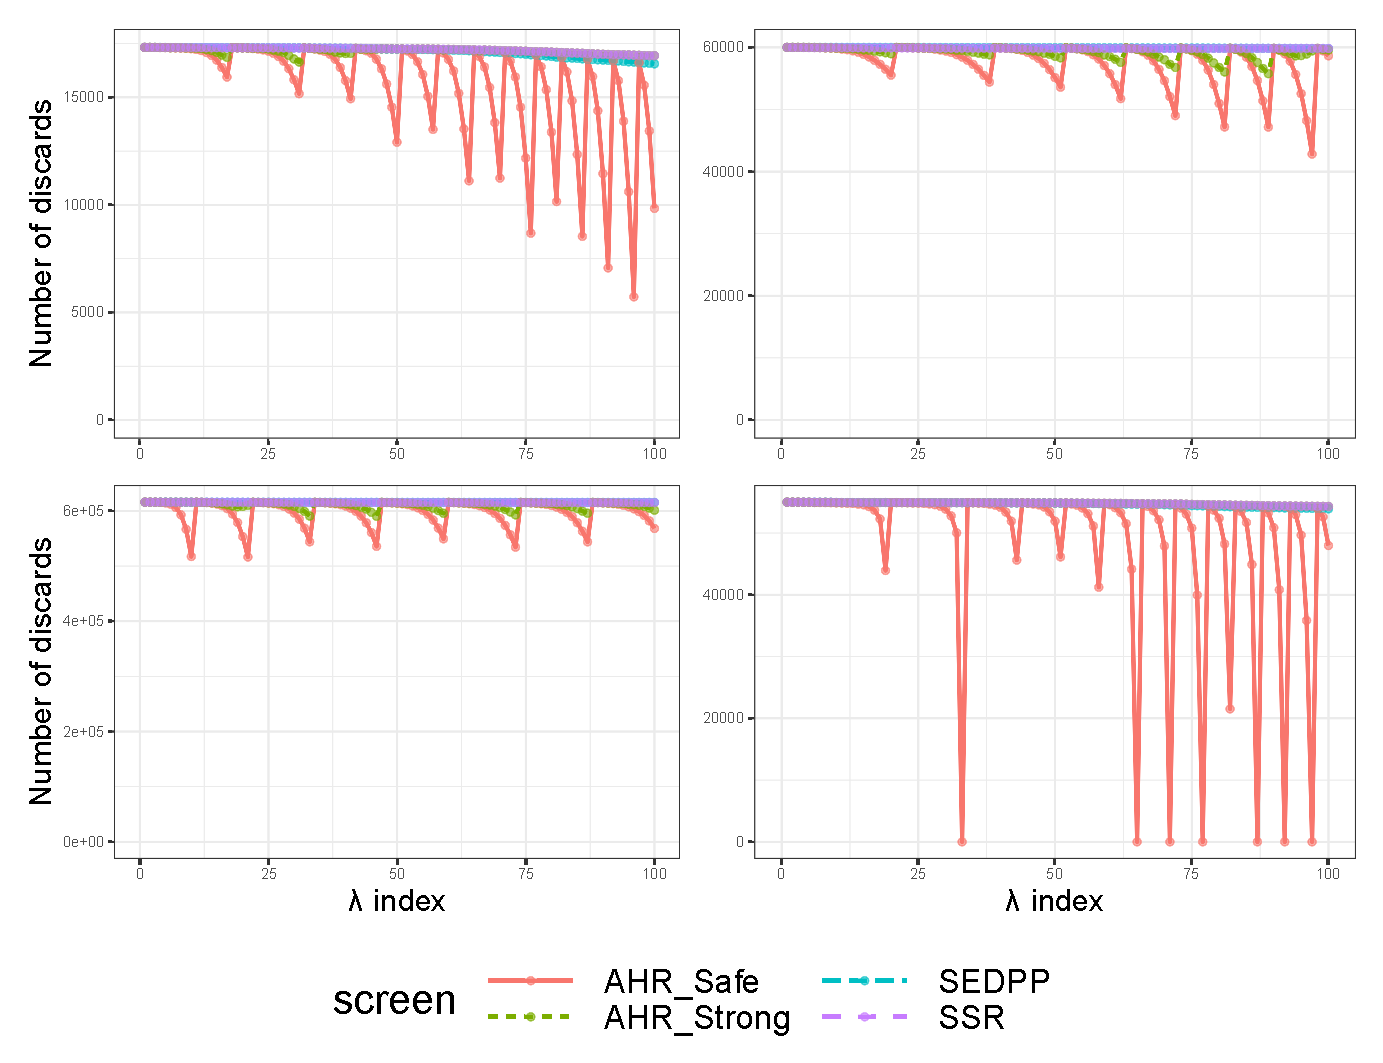
\includegraphics[width=0.82\textwidth]{app1.eps}    \caption{Comparing number of discards by screening methods for lasso model along $\lambda$ values.}
    \label{fig:ap1}
\end{figure}

Note each jump of the number of discards for AHR method indicates an update of reference because a newer reference leads to higher screening power. Our adaptive updating algorithm determines the timing of update dynamically depending on the screening performance. For all four data sets, with about only 10 updates, the adaptive hybrid screening can safely discard a great number of features at most $\lambda$ values.

Next we compare the number of rounds of KKT conditions checks and the number of KKT conditions checks on individual features, needed for AHR and SSR respectively, as shown in Table \ref{Tab:kkt1} and Table \ref{Tab:kkt2}. In a round of KKT conditions check, all features that are not discarded by the safe rule are checked, and a round a KKT conditions check potentially include a large number of KKT conditions checks on individual features. 

\begin{table}[H]
\centering
\begin{tabular}{lllll}
\toprule
Screening method & GENE & MNIST & GWAS & NYT \\
\midrule
SSR & 99 & 99 & 99 & 99 \\
AHR & 99 & 99 & 99 & 99 \\
\bottomrule
\end{tabular}
\caption{Number of rounds of KKT conditions checks required for the whole path}
\label{Tab:kkt1}
\end{table}

\begin{table}[H]
\centering
\begin{tabular}{lllll}
\toprule
Screening method & GENE & MNIST & GWAS & NYT \\
\midrule
SSR & 1,712 & 5,943 & 60,986 & 5,429 \\
AHR & 172 & 286 & 2,353 & 622 \\
\bottomrule
\end{tabular}
\caption{Number of KKT conditions checks on individual features ($\times10^3$) required for the whole path}
\label{Tab:kkt2}
\end{table}

Although a path include $L=100$ $\lambda$ values, the solution at the first value $\lambda_{0}$ is trivially $\hat{\beta}(\lambda_0)=0$ so we are essentially solving along $99$ $\lam$ values. If the strong rule does not make a violation, the minimal number of rounds of KKT conditions checks required will be $99$. In all four data sets, neither SSR nor the adaptive SSR in AHR ever makes a violation. However two methods are very different in terms of the number of KKT conditions checks on individual features, which proportionally increases the computational cost. AHR requires much less checks on individual features because the adaptive EDPP narrows down the set of features that need to be checked by a magnitude.

\end{document}
